% задание и сама лабораторная работа
% Для листинга кода:
\lstset{ %
	language=lisp,                 % выбор языка для подсветки (здесь это С++)
	basicstyle=\small\sffamily, % размер и начертание шрифта для подсветки кода
	numbers=left,               % где поставить нумерацию строк (слева\справа)
	numberstyle=\tiny,           % размер шрифта для номеров строк
	stepnumber=1,                   % размер шага между двумя номерами строк
	numbersep=5pt,                % как далеко отстоят номера строк от подсвечиваемого кода
	showspaces=false,            % показывать или нет пробелы специальными отступами
	showstringspaces=false,      % показывать или нет пробелы в строках
	showtabs=false,             % показывать или нет табуляцию в строках
	frame=single,              % рисовать рамку вокруг кода
	tabsize=2,                 % размер табуляции по умолчанию равен 2 пробелам
	captionpos=t,              % позиция заголовка вверху [t] или внизу [b] 
	breaklines=true,           % автоматически переносить строки (да\нет)
	breakatwhitespace=false, % переносить строки только если есть пробел
	escapeinside={\#*}{*)}   % если нужно добавить комментарии в коде
}
\newpage
\section*{Листинг кода}
\addcontentsline{toc}{section}{\tocsecindent{Листинг кода}}

\begin{lstlisting}
#include <linux/init.h>
#include <linux/module.h>
#include <linux/kernel.h>
#include <linux/pagemap.h> 	/* PAGE_CACHE_SIZE */
#include <linux/fs.h>     	/* This is where libfs stuff is declared */	#include <asm/atomic.h>	
#include <asm/uaccess.h>	/* copy_to_user */
#include <linux/slab.h>
	
MODULE_LICENSE("GPL");
MODULE_AUTHOR("Furdik");
MODULE_DESCRIPTION("Lab8");
	
#define VFS_MAGIC_NUMBER 0x13131313
#define SLABNAME "vfs_cache"
	
static int size = 7;
module_param(size, int, 0);
static int number = 31;
module_param(number, int, 0);
	
static void* obj = NULL;
	
static void co(void* p)
{
	*(int*)p = (int)p;
}

struct kmem_cache *cache = NULL;

static struct vfs_inode
{
	int i_mode;
	unsigned long i_ino;
} vfs_inode;
	
static struct inode * vfs_make_inode(struct super_block *sb, int mode)
{
	struct inode *ret = new_inode(sb);
	if (ret)
	{
		inode_init_owner(ret, NULL, mode);
		ret->i_size = PAGE_SIZE;
		ret->i_atime = ret->i_mtime = ret->i_ctime = current_time(ret);
		ret->i_private = &vfs_inode;
	}
	
	return ret;	
}
	
static void vfs_put_super(struct super_block *sb)
{
	printk(KERN_DEBUG "VFS super block destroyed!\n");
}
	
static struct super_operations const vfs_super_ops = {
	.put_super = vfs_put_super,
	.statfs = simple_statfs,
	.drop_inode = generic_delete_inode,
};
	
static int vfs_fill_sb(struct super_block *sb, void *data, int silent)
{
	struct inode* root = NULL;
		
	sb->s_blocksize = PAGE_SIZE;
	sb->s_blocksize_bits = PAGE_SHIFT;
	sb->s_magic = VFS_MAGIC_NUMBER;
	sb->s_op = &vfs_super_ops;
		

	root = vfs_make_inode(sb, S_IFDIR | 0755);
	if (!root)
	{
		printk (KERN_ERR "VFS inode allocation failed !\n");
		return -ENOMEM;
	}
		
	root->i_op = &simple_dir_inode_operations;
	root->i_fop = &simple_dir_operations;
	
	sb->s_root = d_make_root(root);
	if (!sb->s_root)
	{
			printk(KERN_ERR "VFS root creation failed!\n");
			iput(root);
			return -ENOMEM;
	}
	
	return 0;
}
	
static struct dentry* vfs_mount(struct file_system_type *type, int flags, const char *dev, void *data)
{
	struct dentry* const entry = mount_nodev(type, flags, data, vfs_fill_sb);
		
	if (IS_ERR(entry))
		printk(KERN_ERR  "VFS mounting failed!\n");
	else
		printk(KERN_DEBUG "VFS mounted!\n");
		
		
	return entry;
}
	
static struct file_system_type vfs_type  =  {
	.owner  =  THIS_MODULE, 
	.name  =  "vfs",
	.mount  =  vfs_mount,
	.kill_sb  =  kill_litter_super, 
	};
	
static int __init vfs_module_init(void)
	{
	
	if (size < 0)
	{
		printk(KERN_ERR "VFS_MODULE invalid sizeof objects\n");
		return -EINVAL;
	}
		
	obj = kmalloc(sizeof(void*), GFP_KERNEL);
	if (!obj)
	{
		printk(KERN_ERR "VFS_MODULE kmalloc error\n");
		kfree(obj);
		return -ENOMEM;
	}
		
	cache = kmem_cache_create(SLABNAME, size, 0, SLAB_HWCACHE_ALIGN, co);
		
	if (!cache)
	{
		printk(KERN_ERR "VFS_MODULE cannot create cache\n");
		kmem_cache_destroy(cache);
		return -ENOMEM;
	}
		
	if (NULL == (obj = kmem_cache_alloc(cache, GFP_KERNEL)))
	{
		printk(KERN_ERR "VFS_MODULE cannot alloc object\n");
		kmem_cache_destroy(cache);
		return -ENOMEM;
	}
		
	printk(KERN_INFO "VFS_MODULE allocate %d objects into slab: %s\n", number, SLABNAME);
	printk(KERN_INFO "VFS_MODULE object size %d bytes, full size %ld bytes\n", size, (long)size *number);
		
	int ret = register_filesystem(&vfs_type);
	if (ret != 0)
	{
		printk(KERN_ERR "VFS_MODULE cannot register filesystem!\n");
		return ret;
	}
		
	printk(KERN_DEBUG "VFS_MODULE loaded!\n");
	return 0;
}
	
static void __exit vfs_module_exit(void)
{
	kmem_cache_free(cache, obj);

	kmem_cache_destroy(cache);
	kfree(obj);
		
	if (unregister_filesystem(&vfs_type) != 0)
	{
		printk(KERN_ERR "VFS_MODULE cannot unregister filesystem!\n");
	}
		
	printk(KERN_DEBUG "VFS_MODULE unloaded!\n");
}
	
module_init(vfs_module_init);
module_exit(vfs_module_exit);
	
\end{lstlisting}
\section*{Результат работы}
\addcontentsline{toc}{section}{\tocsecindent{Результат работы}}
1. Скомпилируем модуль ядра и загрузим его, проверив его в списке загруженных модулей ядра.
\begin{figure}[h!]
	\center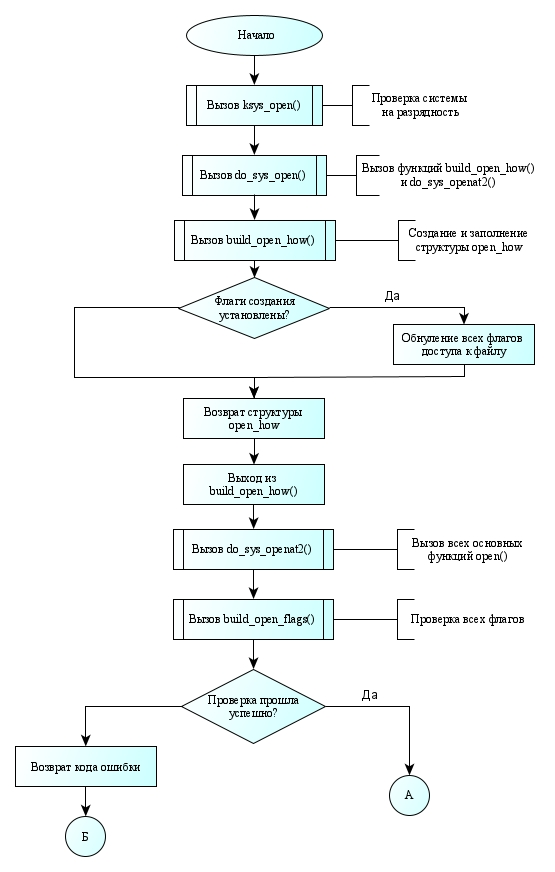
\includegraphics[scale=1]{1.jpg}
\end{figure}
\begin{figure}[h!]
	\center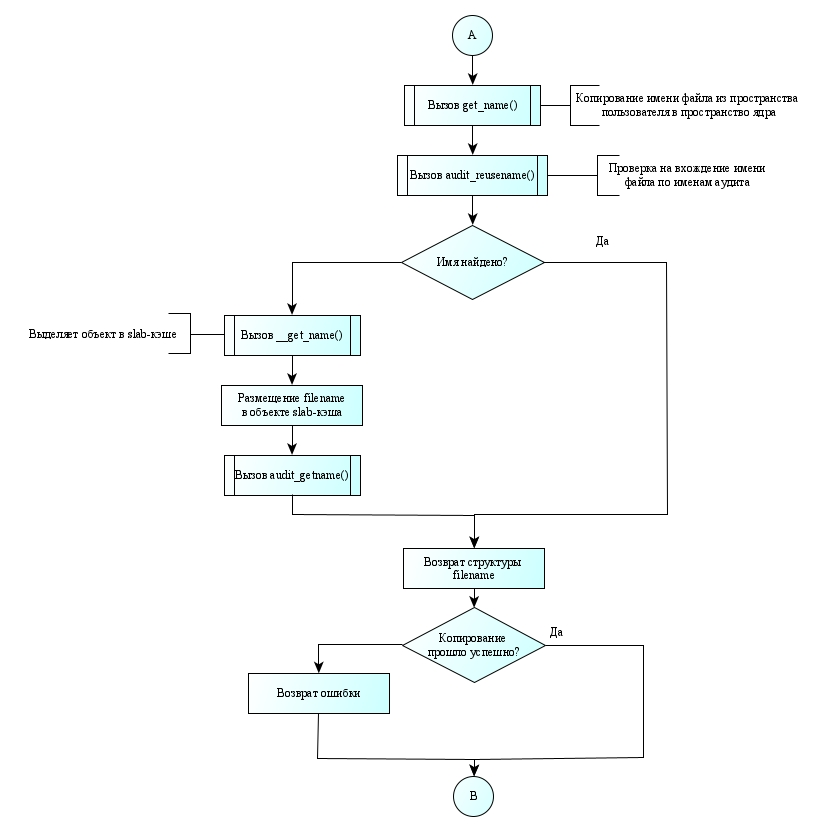
\includegraphics[scale=1]{2.jpg}
\end{figure}
\newline 2. Выведем содержание буфера сообщений ядра, а также проверим содержимое файла /proc/slabinfo, в котором хранится информация о кэшах.
\begin{figure}[h!]
	\center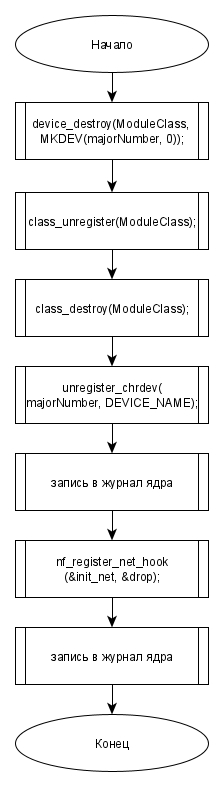
\includegraphics[scale=1]{4.jpg}
\end{figure}
\begin{figure}[h!]
	\center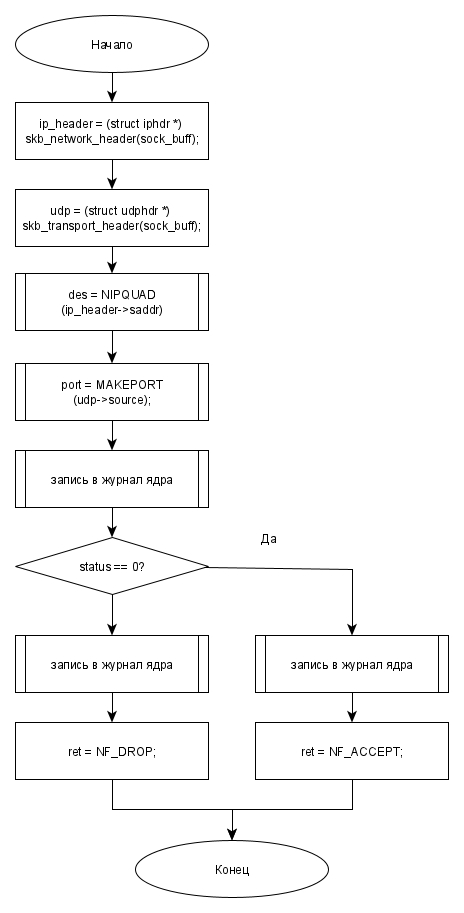
\includegraphics[scale=1]{3.jpg}
\end{figure}
\newline 3. Создадим образ диска. Кроме того, нужно создать каталог, который будет точкой монтирования (корнем) файловой системы. Далее, используя этот образ, примонтируем файловую систему. Проверим успешное монтирование, для чего выведем содержания буфера сообщений ядра.
\newpage 
\begin{figure}[h!]
	\center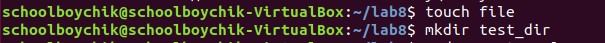
\includegraphics[scale=1]{5.jpg}
\end{figure}
\begin{figure}[h!]
	\center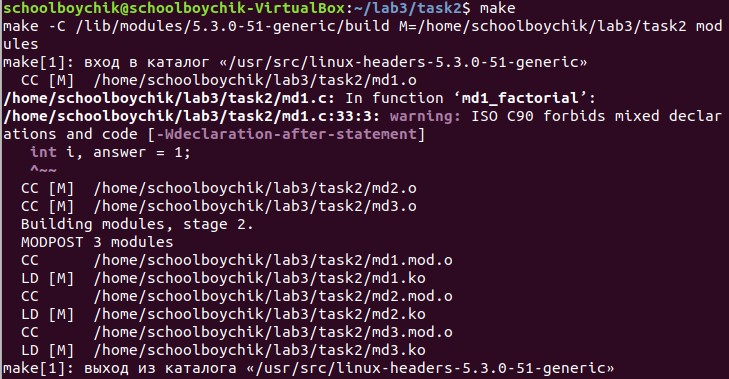
\includegraphics[scale=1]{6.jpg}
\end{figure}
4. Покажем созданную ФС в дереве каталогов
\begin{figure}[h!]
	\center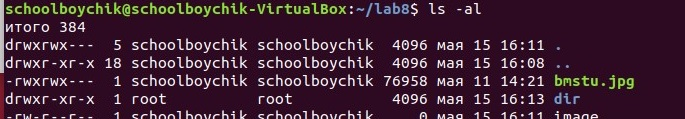
\includegraphics[scale=1]{12.jpg}
\end{figure}
\newline При этом она также отобразилась в проводнике:
\begin{figure}[h!]
	\center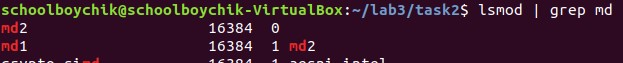
\includegraphics[scale=1]{11.jpg}	
\end{figure}
\newline 5. Размонтируем ФС и выгрузим модуль ядра, также проверив, что выгрузка прошла успешно (для чего выведем содержание буфера сообщений ядра).
\begin{figure}[h!]
	\center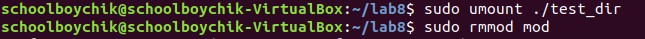
\includegraphics[scale=1]{7.jpg}
\end{figure}
\begin{figure}[h!]
	\center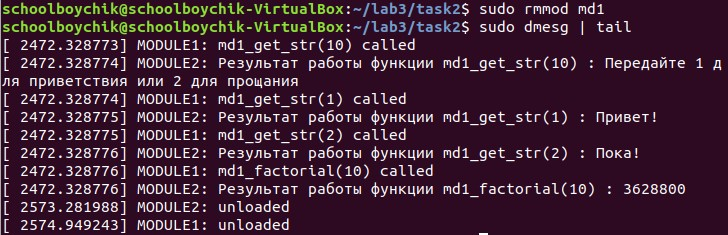
\includegraphics[scale=1]{8.jpg}
\end{figure}
\newline 6. Также продемонстрируем загрузку модуля ядра с заданными размером и количеством элементов кэша.
\begin{figure}[h!]
	\center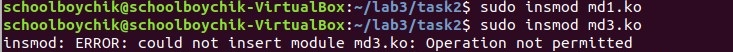
\includegraphics[scale=1]{9.jpg}
\end{figure}
\begin{figure}[h!]
	\center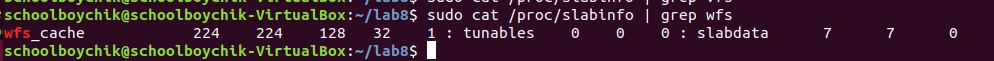
\includegraphics[scale=0.85]{10.jpg}
\end{figure}